\documentclass[12pt]{article}
\usepackage{fontspec}
\usepackage{fullpage}
\usepackage{hyperref}
\hypersetup{bookmarks=true,colorlinks=true,linkcolor=red,citecolor=blue,filecolor=magenta,urlcolor=cyan}
\usepackage{amsmath}
\usepackage{amssymb}
\usepackage{mathtools}
\usepackage{unicode-math}
\usepackage{tabu}
\usepackage{longtable}
\usepackage{booktabs}
\usepackage{caption}
\usepackage{enumitem}
\usepackage{graphics}
\usepackage{filecontents}
\usepackage[backend=bibtex]{biblatex}
\usepackage{url}
\setmathfont{Latin Modern Math}
\newcommand{\gt}{\ensuremath >}
\newcommand{\lt}{\ensuremath <}
\global\tabulinesep=1mm
\newlist{symbDescription}{description}{1}
\setlist[symbDescription]{noitemsep, topsep=0pt, parsep=0pt, partopsep=0pt}
\bibliography{bibfile}
\title{Software Requirements Specification for Truss}
\author{Ting-Yu Wu}
\begin{document}
\maketitle
\tableofcontents
\newpage
\section{Reference Material}
\label{Sec:RefMat}
This section records information for easy reference.

\subsection{Table of Units}
\label{Sec:ToU}
The unit system used throughout is SI (Système International d'Unités). In addition to the basic units, several derived units are also used. For each unit, \hyperref[Table:ToU]{Tab: ToU} lists the symbol, a description and the SI name.

\begin{longtable}{l l l}
\toprule
\textbf{Symbol} & \textbf{Description} & \textbf{SI Name}
\\
\midrule
\endhead
${\text{m}}$ & length & metre
\\
${\text{N}}$ & force & newton
\\
${\text{rad}}$ & angle & radian
\\
\bottomrule
\caption{Table of Units}
\label{Table:ToU}
\end{longtable}
\subsection{Table of Symbols}
\label{Sec:ToS}
The symbols used in this document are summarized in \hyperref[Table:ToS]{Tab: ToS} along with their units. Throughout the document, symbols in bold will represent vectors, and scalars otherwise. The symbols are listed in alphabetical order. For vector quantities, the units shown are for each component of the vector.

\begin{longtable}{l l l}
\toprule
\textbf{Symbol} & \textbf{Description} & \textbf{Units}
\\
\midrule
\endhead
${d_{\text{max}}}$ & Maximum value for distance & ${\text{m}}$
\\
${d_{\text{min}}}$ & Minimum value for distance & ${\text{m}}$
\\
${\mathbf{F}_{1}}$ & External force & ${\text{N}}$
\\
${\mathbf{F}_{\text{AC}}}$ & Force between joint A and C & ${\text{N}}$
\\
${\mathbf{F}_{\text{AD}}}$ & Force between joint A and D & ${\text{N}}$
\\
${\mathbf{F}_{\text{Ax}}}$ & X-component of reaction force on joint A & ${\text{N}}$
\\
${\mathbf{F}_{\text{Ay}}}$ & Y-component of reaction force on joint A & ${\text{N}}$
\\
${\mathbf{F}_{\text{BC}}}$ & Force between joint B and C & ${\text{N}}$
\\
${\mathbf{F}_{\text{BD}}}$ & Force between joint B and D & ${\text{N}}$
\\
${\mathbf{F}_{\text{By}}}$ & Y-component of reaction force on joint B & ${\text{N}}$
\\
${\mathbf{F}_{\text{CD}}}$ & Force between joint C and D & ${\text{N}}$
\\
${\mathbf{F}_{\text{max}}}$ & Maximum value for external force & ${\text{N}}$
\\
${\mathbf{F}_{\text{min}}}$ & Minimum value for external force & ${\text{N}}$
\\
${\mathbf{F}_{\text{out}}}$ & All the output forces & ${\text{N}}$
\\
${\mathbf{F}_{\text{x}}}$ & Force component in the x direction & ${\text{N}}$
\\
${\mathbf{F}_{\text{y}}}$ & Force component in the y direction & ${\text{N}}$
\\
${\mathbf{M}_{\text{i}}}$ & Moment component of joint i & $\text{N}\text{m}$
\\
${x_{\text{1}}}$ & Distance from joint A to joint D & ${\text{m}}$
\\
${x_{\text{2}}}$ & Distance from joint D to joint B & ${\text{m}}$
\\
${θ_{\text{1}}}$ & Angle between member 1 and 3 & ${\text{rad}}$
\\
${θ_{\text{2}}}$ & Angle between member 2 and 4 & ${\text{rad}}$
\\
${θ_{\text{max}}}$ & Maximum value for angle & ${\text{rad}}$
\\
${θ_{\text{min}}}$ & Minimum value for angle & ${\text{rad}}$
\\
$π$ & Ratio of circumference to diameter for any circle & --
\\
\bottomrule
\caption{Table of Symbols}
\label{Table:ToS}
\end{longtable}
\subsection{Abbreviations and Acronyms}
\label{Sec:TAbbAcc}
\begin{longtable}{l l}
\toprule
\textbf{Abbreviation} & \textbf{Full Form}
\\
\midrule
\endhead
A & Assumption
\\
DD & Data Definition
\\
GD & General Definition
\\
GS & Goal Statement
\\
IM & Instance Model
\\
LC & Likely Change
\\
PS & Physical System Description
\\
R & Requirement
\\
SRS & Software Requirements Specification
\\
TM & Theoretical Model
\\
UC & Unlikely Change
\\
\bottomrule
\caption{Abbreviations and Acronyms}
\label{Table:TAbbAcc}
\end{longtable}
\section{Introduction}
\label{Sec:Intro}
Truss analysis is a common problem in mechanics. Therefore, it is useful to have a program to solve and model these types of problems. The program documented here is called Truss.

The following section provides an overview of the Software Requirements Specification (SRS) for Truss. This section explains the purpose of this document, the scope of the requirements, the characteristics of the intended reader, and the organization of the document.

\subsection{Scope of Requirements}
\label{Sec:ReqsScope}
The scope of the requirements includes solving for unknown forces and find out their stress distribution of a ideal Truss structure.

\section{Specific System Description}
\label{Sec:SpecSystDesc}
This section first presents the problem description, which gives a high-level view of the problem to be solved. This is followed by the solution characteristics specification, which presents the assumptions, theories, and definitions that are used.

\subsection{Problem Description}
\label{Sec:ProbDesc}
A system is needed to analyze the unknown forces acting on truss.

\subsubsection{Terminology and Definitions}
\label{Sec:TermDefs}
This subsection provides a list of terms that are used in the subsequent sections and their meaning, with the purpose of reducing ambiguity and making it easier to correctly understand the requirements.

\begin{itemize}
\item{Compression: The force that squeezes materials together.}
\item{Force Equilibrium: A body is in force equilibrium if the sum of all the forces acting on the body is zero.}
\item{Joint: A place where two trusses are connected.}
\item{Method of Joint: A way to find unknown forces in a truss structure. The principle behind this method is that all forces acting on a joint must add to zero.}
\item{Moment: Moment of a force, also called torque, is the tendency to cause a body to rotate about a specific point or axis.}
\item{Moment Equilibrium: A body is in moment equilibrium if the sum of all the moments of all the forces acting on the body is zero.}
\item{Pin Support: A kind of structural support can have both a horizontal x direction force and a vertical y direction force.}
\item{Reaction Force: An external force on a body which is contributed by its supports or connections.}
\item{Roller Support: A kind of structural support can only have a vertical y direction force.}
\item{Tension: The force that pulls materials apart.}
\end{itemize}
\subsubsection{Physical System Description}
\label{Sec:PhysSyst}
The physical system of Truss, as shown in \hyperref[Figure:physSysImage]{Fig:physSysImage}, includes the following elements:

\begin{itemize}
\item[PS1:]{The pin support.}
\item[PS2:]{The roller support.}
\item[PS3:]{The joints.}
\item[PS4:]{Truss members.}
\end{itemize}
\begin{figure}
\begin{center}
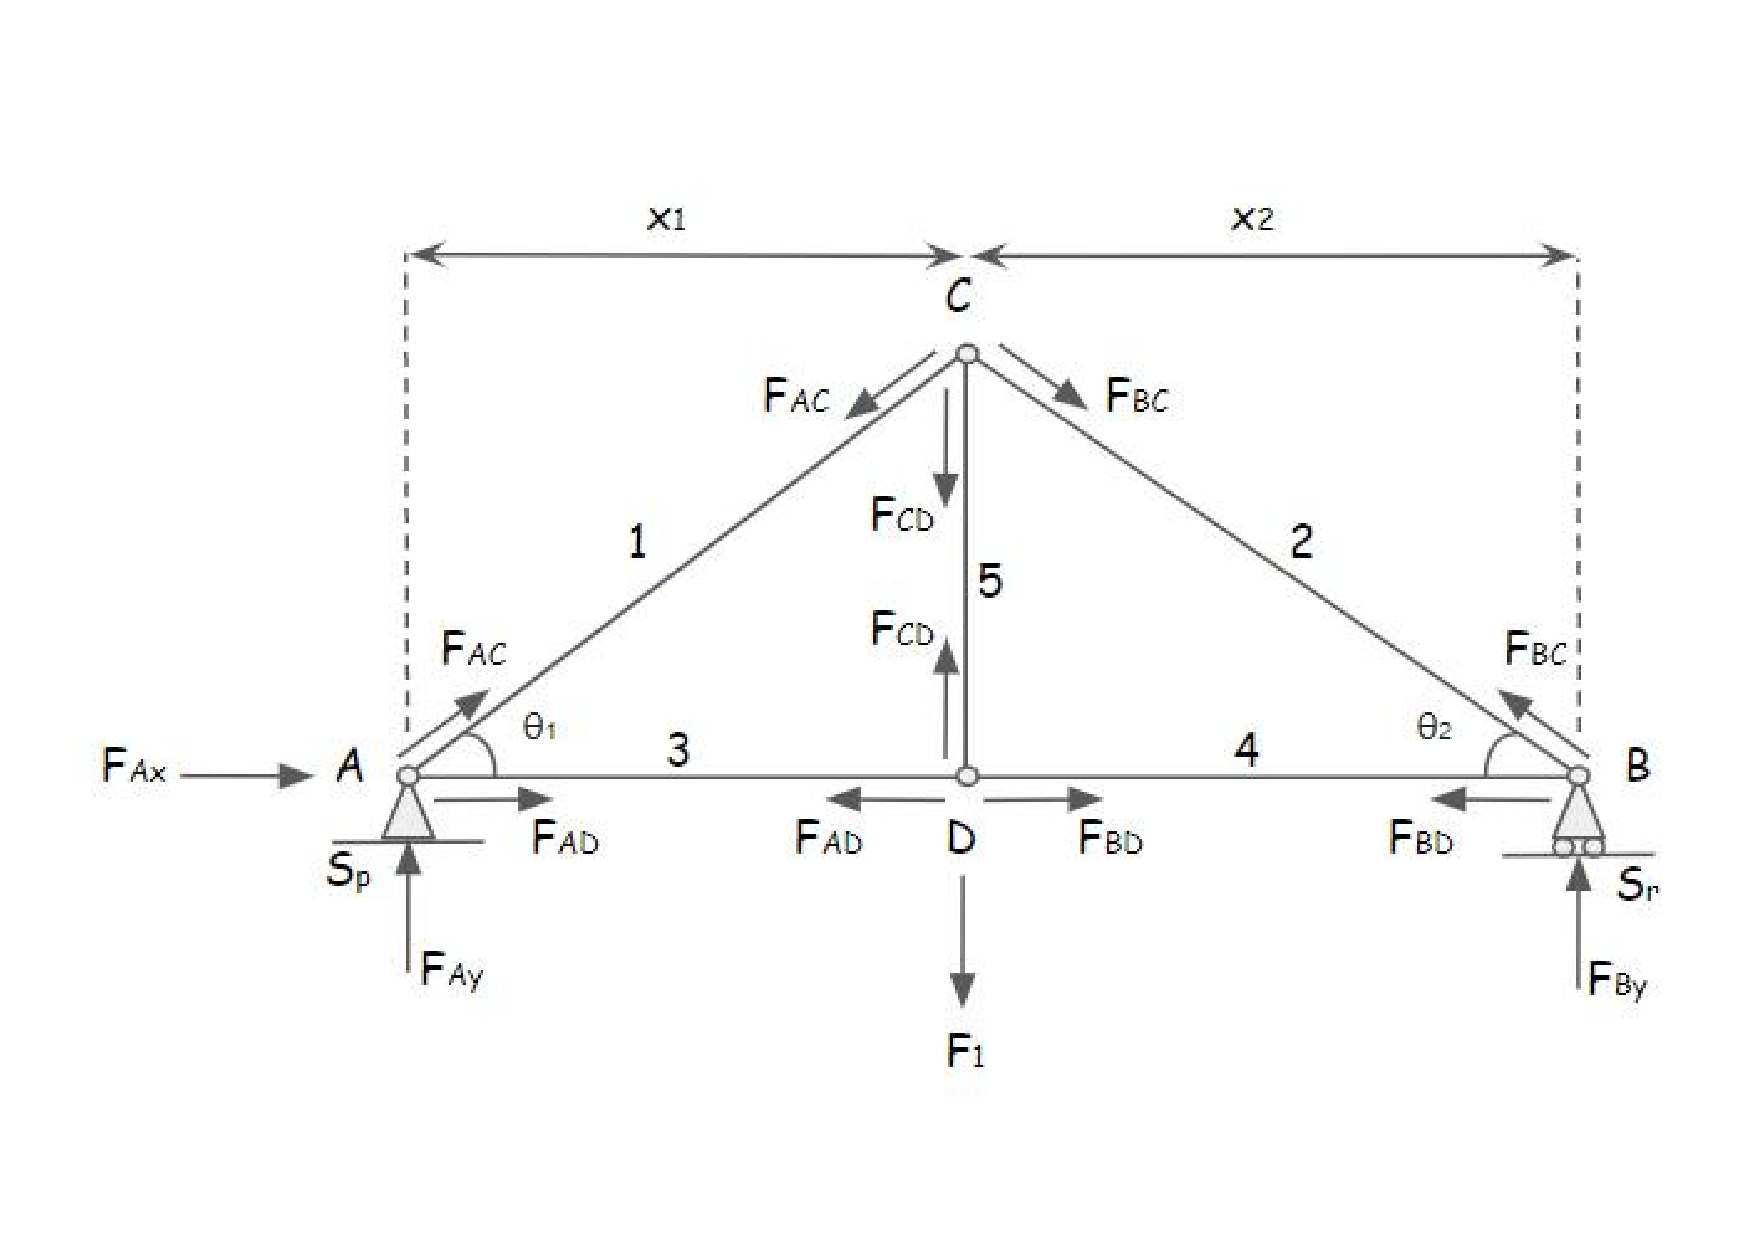
\includegraphics[width=0.7\textwidth]{../../../datafiles/Truss/PhysicalSystem.png}
\caption{The physical system}
\label{Figure:physSysImage}
\end{center}
\end{figure}
\subsubsection{Goal Statements}
\label{Sec:GoalStmt}
Given truss properties and the external force, the goal statements are:

\begin{itemize}
\item[reactionForce:\phantomsection\label{reactionForce}]{Solve the support reaction forces.}
\item[internalForce:\phantomsection\label{internalForce}]{Solve the internal forces acting on truss members.}
\end{itemize}
\subsection{Solution Characteristics Specification}
\label{Sec:SolCharSpec}
The instance models that govern Truss are presented in \hyperref[Sec:IMs]{Section: Instance Models}. The information to understand the meaning of the instance models and their derivation is also presented, so that the instance models can be verified.

\subsubsection{Assumptions}
\label{Sec:Assumps}
This section simplifies the original problem and helps in developing the theoretical models by filling in the missing information for the physical system. The assumptions refine the scope by providing more detail.

\begin{itemize}
\item[staticDeterminate:\phantomsection\label{staticDeterminate}]{The structure is statically determinate. (RefBy: \hyperref[unlikeChgStatD]{UC: Statically-Determinate} and \hyperref[TM:staticEquilibrium]{TM: staticEquilibrium}.)}
\item[pinConnected:\phantomsection\label{pinConnected}]{All joints are connected by frictionless pins. (RefBy: \hyperref[IM:reactionAy]{IM: reactionAy}, \hyperref[IM:reactionAx]{IM: reactionAx}, and \hyperref[likeChgNCbP]{LC: Not-Connected-by-Pin}.)}
\item[connectedatEnd:\phantomsection\label{connectedatEnd}]{Truss members are connected only at their end.}
\item[straightTruss:\phantomsection\label{straightTruss}]{All the truss members are perfectly straight. (RefBy: \hyperref[unlikeChgST]{UC: Straight-Truss}.)}
\item[igWeight:\phantomsection\label{igWeight}]{The weight of the members are negligibly small which can be ignored. (RefBy: \hyperref[likeChgWoT]{LC: Consider-Truss-Weight}.)}
\item[twokindForce:\phantomsection\label{twokindForce}]{All the members have only tension or compression force. (RefBy: \hyperref[likeChgOtherF]{LC: Other-Forces-Involved}.)}
\item[applyatJoint:\phantomsection\label{applyatJoint}]{All loads and support reactions are applied at the joints only.}
\end{itemize}
\subsubsection{Theoretical Models}
\label{Sec:TMs}
This section focuses on the general equations and laws that Truss is based on.

\vspace{\baselineskip}
\noindent
\begin{minipage}{\textwidth}
\begin{tabular}{>{\raggedright}p{0.13\textwidth}>{\raggedright\arraybackslash}p{0.82\textwidth}}
\toprule \textbf{Refname} & \textbf{TM:staticEquilibrium}
\phantomsection 
\label{TM:staticEquilibrium}
\\ \midrule \\
Label & Static Equilibrium
        
\\ \midrule \\
Equation & \begin{displaymath}
           \displaystyle\sum{{\mathbf{F}_{\text{x}}}={\mathbf{F}_{\text{y}}}={\mathbf{M}_{\text{i}}}=0}
           \end{displaymath}
\\ \midrule \\
Description & \begin{symbDescription}
              \item{${\mathbf{F}_{\text{x}}}$ is the force component in the x direction (${\text{N}}$)}
              \item{${\mathbf{F}_{\text{y}}}$ is the force component in the y direction (${\text{N}}$)}
              \item{${\mathbf{M}_{\text{i}}}$ is the moment component of joint i ($\text{N}\text{m}$)}
              \end{symbDescription}
\\ \midrule \\
Notes & The structure is assumed to be statically determinate (from \hyperref[staticDeterminate]{A: staticDeterminate}).
        
\\ \midrule \\
Source & \cite{mofjWiki} and \cite{momentWiki}
         
\\ \midrule \\
RefBy & \hyperref[IM:reactionBy]{IM: reactionBy}, \hyperref[IM:reactionAy]{IM: reactionAy}, \hyperref[IM:reactionAx]{IM: reactionAx}, \hyperref[IM:internalCD]{IM: internalCD}, \hyperref[IM:internalBD]{IM: internalBD}, \hyperref[IM:internalBC]{IM: internalBC}, \hyperref[IM:internalAD]{IM: internalAD}, and \hyperref[IM:internalAC]{IM: internalAC}
        
\\ \bottomrule
\end{tabular}
\end{minipage}
\subsubsection{Instance Models}
\label{Sec:IMs}
This section transforms the problem defined in \hyperref[Sec:ProbDesc]{Section: Problem Description} into one which is expressed in mathematical terms. It uses concrete symbols defined in \hyperref[Sec:DDs]{Section: Data Definitions} to replace the abstract symbols in the models identified in \hyperref[Sec:TMs]{Section: Theoretical Models} and \hyperref[Sec:GDs]{Section: General Definitions}.

\vspace{\baselineskip}
\noindent
\begin{minipage}{\textwidth}
\begin{tabular}{>{\raggedright}p{0.13\textwidth}>{\raggedright\arraybackslash}p{0.82\textwidth}}
\toprule \textbf{Refname} & \textbf{IM:reactionAx}
\phantomsection 
\label{IM:reactionAx}
\\ \midrule \\
Label & Support reaction force on joint A in the x direction
        
\\ \midrule \\
Input & 
\\ \midrule \\
Output & ${\mathbf{F}_{\text{Ax}}}$
         
\\ \midrule \\
Input Constraints & 
\\ \midrule \\
Output Constraints & 
\\ \midrule \\
Equation & \begin{displaymath}
           {\mathbf{F}_{\text{Ax}}}=0
           \end{displaymath}
\\ \midrule \\
Description & \begin{symbDescription}
              \item{${\mathbf{F}_{\text{Ax}}}$ is the x-component of reaction force on joint A (${\text{N}}$)}
              \end{symbDescription}
\\ \midrule \\
Notes & There is a reacting force in the x direction, ${\mathbf{F}_{\text{Ax}}}$ , since joint A is pinned (from \hyperref[pinConnected]{A: pinConnected}). We apply the static equilibrium to slove the reaction force (from \hyperref[TM:staticEquilibrium]{TM: staticEquilibrium})..
        
\\ \midrule \\
Source & --
         
\\ \midrule \\
RefBy & \hyperref[calcValues]{FR: Calculate-Values}
        
\\ \bottomrule
\end{tabular}
\end{minipage}

\vspace{\baselineskip}
\noindent
\begin{minipage}{\textwidth}
\begin{tabular}{>{\raggedright}p{0.13\textwidth}>{\raggedright\arraybackslash}p{0.82\textwidth}}
\toprule \textbf{Refname} & \textbf{IM:reactionAy}
\phantomsection 
\label{IM:reactionAy}
\\ \midrule \\
Label & Support reaction force on joint A in the y direction
        
\\ \midrule \\
Input & ${\mathbf{F}_{1}}$, ${x_{\text{1}}}$, ${x_{\text{2}}}$
        
\\ \midrule \\
Output & ${\mathbf{F}_{\text{Ay}}}$
         
\\ \midrule \\
Input Constraints & \begin{displaymath}
                    {x_{\text{1}}}\gt{}0
                    \end{displaymath}
                    \begin{displaymath}
                    {x_{\text{2}}}\gt{}0
                    \end{displaymath}
\\ \midrule \\
Output Constraints & 
\\ \midrule \\
Equation & \begin{displaymath}
           {\mathbf{F}_{\text{Ay}}}=\frac{{\mathbf{F}_{1}} {x_{\text{2}}}}{{x_{\text{1}}}+{x_{\text{2}}}}
           \end{displaymath}
\\ \midrule \\
Description & \begin{symbDescription}
              \item{${\mathbf{F}_{\text{Ay}}}$ is the y-component of reaction force on joint A (${\text{N}}$)}
              \item{${\mathbf{F}_{1}}$ is the external force (${\text{N}}$)}
              \item{${x_{\text{2}}}$ is the distance from joint D to joint B (${\text{m}}$)}
              \item{${x_{\text{1}}}$ is the distance from joint A to joint D (${\text{m}}$)}
              \end{symbDescription}
\\ \midrule \\
Notes & There is a reacting force in the y direction, ${\mathbf{F}_{\text{Ay}}}$ , since joint A is pinned (from \hyperref[pinConnected]{A: pinConnected}). We apply the static equilibrium to slove the reaction force (from \hyperref[TM:staticEquilibrium]{TM: staticEquilibrium})..
        
        ${x_{\text{1}}}$ and ${x_{\text{2}}}$ are shown in \hyperref[Figure:physSysImage]{Fig:physSysImage}..
        
\\ \midrule \\
Source & --
         
\\ \midrule \\
RefBy & \hyperref[IM:internalAC]{IM: internalAC} and \hyperref[calcValues]{FR: Calculate-Values}
        
\\ \bottomrule
\end{tabular}
\end{minipage}

\vspace{\baselineskip}
\noindent
\begin{minipage}{\textwidth}
\begin{tabular}{>{\raggedright}p{0.13\textwidth}>{\raggedright\arraybackslash}p{0.82\textwidth}}
\toprule \textbf{Refname} & \textbf{IM:reactionBy}
\phantomsection 
\label{IM:reactionBy}
\\ \midrule \\
Label & Support reaction force on joint B in the y direction
        
\\ \midrule \\
Input & ${\mathbf{F}_{1}}$, ${x_{\text{1}}}$, ${x_{\text{2}}}$
        
\\ \midrule \\
Output & ${\mathbf{F}_{\text{By}}}$
         
\\ \midrule \\
Input Constraints & \begin{displaymath}
                    {x_{\text{1}}}\gt{}0
                    \end{displaymath}
                    \begin{displaymath}
                    {x_{\text{2}}}\gt{}0
                    \end{displaymath}
\\ \midrule \\
Output Constraints & 
\\ \midrule \\
Equation & \begin{displaymath}
           {\mathbf{F}_{\text{By}}}=\frac{{\mathbf{F}_{1}} {x_{\text{1}}}}{{x_{\text{1}}}+{x_{\text{2}}}}
           \end{displaymath}
\\ \midrule \\
Description & \begin{symbDescription}
              \item{${\mathbf{F}_{\text{By}}}$ is the y-component of reaction force on joint B (${\text{N}}$)}
              \item{${\mathbf{F}_{1}}$ is the external force (${\text{N}}$)}
              \item{${x_{\text{1}}}$ is the distance from joint A to joint D (${\text{m}}$)}
              \item{${x_{\text{2}}}$ is the distance from joint D to joint B (${\text{m}}$)}
              \end{symbDescription}
\\ \midrule \\
Notes & We apply the static equilibrium to slove the reaction force (from \hyperref[TM:staticEquilibrium]{TM: staticEquilibrium})..
        
        ${x_{\text{1}}}$ and ${x_{\text{2}}}$ are shown in \hyperref[Figure:physSysImage]{Fig:physSysImage}..
        
\\ \midrule \\
Source & --
         
\\ \midrule \\
RefBy & \hyperref[IM:internalBC]{IM: internalBC} and \hyperref[calcValues]{FR: Calculate-Values}
        
\\ \bottomrule
\end{tabular}
\end{minipage}

\vspace{\baselineskip}
\noindent
\begin{minipage}{\textwidth}
\begin{tabular}{>{\raggedright}p{0.13\textwidth}>{\raggedright\arraybackslash}p{0.82\textwidth}}
\toprule \textbf{Refname} & \textbf{IM:internalAC}
\phantomsection 
\label{IM:internalAC}
\\ \midrule \\
Label & Solving internal force between joint A and C
        
\\ \midrule \\
Input & ${\mathbf{F}_{\text{Ay}}}$, ${θ_{\text{1}}}$
        
\\ \midrule \\
Output & ${\mathbf{F}_{\text{AC}}}$
         
\\ \midrule \\
Input Constraints & \begin{displaymath}
                    {θ_{\text{1}}}\gt{}0
                    \end{displaymath}
\\ \midrule \\
Output Constraints & 
\\ \midrule \\
Equation & \begin{displaymath}
           {\mathbf{F}_{\text{AC}}}=-\left(\frac{{\mathbf{F}_{\text{Ay}}}}{\sin\left({θ_{\text{1}}}\right)}\right)
           \end{displaymath}
\\ \midrule \\
Description & \begin{symbDescription}
              \item{${\mathbf{F}_{\text{AC}}}$ is the force between joint A and C (${\text{N}}$)}
              \item{${\mathbf{F}_{\text{Ay}}}$ is the y-component of reaction force on joint A (${\text{N}}$)}
              \item{${θ_{\text{1}}}$ is the angle between member 1 and 3 (${\text{rad}}$)}
              \end{symbDescription}
\\ \midrule \\
Notes & $\displaystyle\sum{{\mathbf{F}_{\text{y}}}={\mathbf{F}_{\text{Ay}}}+{\mathbf{F}_{\text{AC}}} \sin\left({θ_{\text{1}}}\right)=0}$ (from \hyperref[TM:staticEquilibrium]{TM: staticEquilibrium})..
        
        ${\mathbf{F}_{\text{Ay}}}$ is from \hyperref[IM:reactionAy]{IM: reactionAy}..
        
        Truss structure is show in \hyperref[Figure:physSysImage]{Fig:physSysImage}.
        
\\ \midrule \\
Source & --
         
\\ \midrule \\
RefBy & \hyperref[outputValues]{FR: Output-Values} and \hyperref[IM:internalAD]{IM: internalAD}
        
\\ \bottomrule
\end{tabular}
\end{minipage}

\vspace{\baselineskip}
\noindent
\begin{minipage}{\textwidth}
\begin{tabular}{>{\raggedright}p{0.13\textwidth}>{\raggedright\arraybackslash}p{0.82\textwidth}}
\toprule \textbf{Refname} & \textbf{IM:internalAD}
\phantomsection 
\label{IM:internalAD}
\\ \midrule \\
Label & Solving internal force between joint A and D
        
\\ \midrule \\
Input & ${\mathbf{F}_{\text{AC}}}$, ${θ_{\text{1}}}$
        
\\ \midrule \\
Output & ${\mathbf{F}_{\text{AD}}}$
         
\\ \midrule \\
Input Constraints & \begin{displaymath}
                    {θ_{\text{1}}}\gt{}0
                    \end{displaymath}
\\ \midrule \\
Output Constraints & 
\\ \midrule \\
Equation & \begin{displaymath}
           {\mathbf{F}_{\text{AD}}}=-\left(\frac{{\mathbf{F}_{\text{AC}}}}{\cos\left({θ_{\text{1}}}\right)}\right)
           \end{displaymath}
\\ \midrule \\
Description & \begin{symbDescription}
              \item{${\mathbf{F}_{\text{AD}}}$ is the force between joint A and D (${\text{N}}$)}
              \item{${\mathbf{F}_{\text{AC}}}$ is the force between joint A and C (${\text{N}}$)}
              \item{${θ_{\text{1}}}$ is the angle between member 1 and 3 (${\text{rad}}$)}
              \end{symbDescription}
\\ \midrule \\
Notes & $\displaystyle\sum{{\mathbf{F}_{\text{x}}}={\mathbf{F}_{\text{AD}}}+{\mathbf{F}_{\text{AC}}} \cos\left({θ_{\text{1}}}\right)=0}$ (from \hyperref[TM:staticEquilibrium]{TM: staticEquilibrium})..
        
        ${\mathbf{F}_{\text{AC}}}$ is from \hyperref[IM:internalAC]{IM: internalAC}..
        
        Truss structure is show in \hyperref[Figure:physSysImage]{Fig:physSysImage}.
        
\\ \midrule \\
Source & --
         
\\ \midrule \\
RefBy & \hyperref[outputValues]{FR: Output-Values}
        
\\ \bottomrule
\end{tabular}
\end{minipage}

\vspace{\baselineskip}
\noindent
\begin{minipage}{\textwidth}
\begin{tabular}{>{\raggedright}p{0.13\textwidth}>{\raggedright\arraybackslash}p{0.82\textwidth}}
\toprule \textbf{Refname} & \textbf{IM:internalBC}
\phantomsection 
\label{IM:internalBC}
\\ \midrule \\
Label & Solving internal force between joint B and C
        
\\ \midrule \\
Input & ${\mathbf{F}_{\text{By}}}$, ${θ_{\text{2}}}$
        
\\ \midrule \\
Output & ${\mathbf{F}_{\text{BC}}}$
         
\\ \midrule \\
Input Constraints & \begin{displaymath}
                    {θ_{\text{2}}}\gt{}0
                    \end{displaymath}
\\ \midrule \\
Output Constraints & 
\\ \midrule \\
Equation & \begin{displaymath}
           {\mathbf{F}_{\text{BC}}}=-\left(\frac{{\mathbf{F}_{\text{By}}}}{\sin\left({θ_{\text{2}}}\right)}\right)
           \end{displaymath}
\\ \midrule \\
Description & \begin{symbDescription}
              \item{${\mathbf{F}_{\text{BC}}}$ is the force between joint B and C (${\text{N}}$)}
              \item{${\mathbf{F}_{\text{By}}}$ is the y-component of reaction force on joint B (${\text{N}}$)}
              \item{${θ_{\text{2}}}$ is the angle between member 2 and 4 (${\text{rad}}$)}
              \end{symbDescription}
\\ \midrule \\
Notes & $\displaystyle\sum{{\mathbf{F}_{\text{y}}}={\mathbf{F}_{\text{By}}}+{\mathbf{F}_{\text{BC}}} \sin\left({θ_{\text{2}}}\right)=0}$ (from \hyperref[TM:staticEquilibrium]{TM: staticEquilibrium})..
        
        ${\mathbf{F}_{\text{By}}}$ is from \hyperref[IM:reactionBy]{IM: reactionBy}..
        
        Truss structure is show in \hyperref[Figure:physSysImage]{Fig:physSysImage}.
        
\\ \midrule \\
Source & --
         
\\ \midrule \\
RefBy & \hyperref[outputValues]{FR: Output-Values} and \hyperref[IM:internalBD]{IM: internalBD}
        
\\ \bottomrule
\end{tabular}
\end{minipage}

\vspace{\baselineskip}
\noindent
\begin{minipage}{\textwidth}
\begin{tabular}{>{\raggedright}p{0.13\textwidth}>{\raggedright\arraybackslash}p{0.82\textwidth}}
\toprule \textbf{Refname} & \textbf{IM:internalBD}
\phantomsection 
\label{IM:internalBD}
\\ \midrule \\
Label & Solving internal force between joint B and D
        
\\ \midrule \\
Input & ${\mathbf{F}_{\text{BC}}}$, ${θ_{\text{2}}}$
        
\\ \midrule \\
Output & ${\mathbf{F}_{\text{BD}}}$
         
\\ \midrule \\
Input Constraints & \begin{displaymath}
                    {θ_{\text{2}}}\gt{}0
                    \end{displaymath}
\\ \midrule \\
Output Constraints & 
\\ \midrule \\
Equation & \begin{displaymath}
           {\mathbf{F}_{\text{BD}}}=-\left(\frac{{\mathbf{F}_{\text{BC}}}}{\cos\left({θ_{\text{2}}}\right)}\right)
           \end{displaymath}
\\ \midrule \\
Description & \begin{symbDescription}
              \item{${\mathbf{F}_{\text{BD}}}$ is the force between joint B and D (${\text{N}}$)}
              \item{${\mathbf{F}_{\text{BC}}}$ is the force between joint B and C (${\text{N}}$)}
              \item{${θ_{\text{2}}}$ is the angle between member 2 and 4 (${\text{rad}}$)}
              \end{symbDescription}
\\ \midrule \\
Notes & $\displaystyle\sum{{\mathbf{F}_{\text{x}}}={\mathbf{F}_{\text{BD}}}+{\mathbf{F}_{\text{BC}}} \cos\left({θ_{\text{2}}}\right)=0}$ (from \hyperref[TM:staticEquilibrium]{TM: staticEquilibrium})..
        
        ${\mathbf{F}_{\text{BC}}}$ is from \hyperref[IM:internalBC]{IM: internalBC}..
        
        Truss structure is show in \hyperref[Figure:physSysImage]{Fig:physSysImage}.
        
\\ \midrule \\
Source & --
         
\\ \midrule \\
RefBy & \hyperref[outputValues]{FR: Output-Values}
        
\\ \bottomrule
\end{tabular}
\end{minipage}

\vspace{\baselineskip}
\noindent
\begin{minipage}{\textwidth}
\begin{tabular}{>{\raggedright}p{0.13\textwidth}>{\raggedright\arraybackslash}p{0.82\textwidth}}
\toprule \textbf{Refname} & \textbf{IM:internalCD}
\phantomsection 
\label{IM:internalCD}
\\ \midrule \\
Label & Solving internal force between joint C and D
        
\\ \midrule \\
Input & ${\mathbf{F}_{1}}$
        
\\ \midrule \\
Output & ${\mathbf{F}_{\text{CD}}}$
         
\\ \midrule \\
Input Constraints & 
\\ \midrule \\
Output Constraints & 
\\ \midrule \\
Equation & \begin{displaymath}
           {\mathbf{F}_{\text{CD}}}={\mathbf{F}_{1}}
           \end{displaymath}
\\ \midrule \\
Description & \begin{symbDescription}
              \item{${\mathbf{F}_{\text{CD}}}$ is the force between joint C and D (${\text{N}}$)}
              \item{${\mathbf{F}_{1}}$ is the external force (${\text{N}}$)}
              \end{symbDescription}
\\ \midrule \\
Notes & $\displaystyle\sum{{\mathbf{F}_{\text{y}}}={\mathbf{F}_{\text{CD}}}-{\mathbf{F}_{1}}=0}$ (from \hyperref[TM:staticEquilibrium]{TM: staticEquilibrium})..
        
        Truss structure is show in \hyperref[Figure:physSysImage]{Fig:physSysImage}.
        
\\ \midrule \\
Source & --
         
\\ \midrule \\
RefBy & \hyperref[outputValues]{FR: Output-Values}
        
\\ \bottomrule
\end{tabular}
\end{minipage}

\subsubsection{Data Constraints}
\label{Sec:DataConstraints}
\hyperref[Table:InDataConstraints]{Table:InDataConstraints} shows the data constraints on the input variables. The column for physical constraints gives the physical limitations on the range of values that can be taken by the variable. The uncertainty column provides an estimate of the confidence with which the physical quantities can be measured. This information would be part of the input if one were performing an uncertainty quantification exercise. The constraints are conservative, to give the user of the model the flexibility to experiment with unusual situations. The column of typical values is intended to provide a feel for a common scenario.

\begin{longtable}{l l l l l}
\toprule
\textbf{Var} & \textbf{Physical Constraints} & \textbf{Software Constraints} & \textbf{Typical Value} & \textbf{Uncert.}
\\
\midrule
\endhead
${\mathbf{F}_{1}}$ & ${\mathbf{F}_{1}}\gt{}0$ & ${\mathbf{F}_{\text{min}}}\leq{}{\mathbf{F}_{1}}\leq{}{\mathbf{F}_{\text{max}}}$ & $500.0$ ${\text{N}}$ & 10$\%$
\\
${x_{\text{1}}}$ & ${x_{\text{1}}}\gt{}0$ & ${d_{\text{min}}}\lt{}{x_{\text{1}}}\leq{}{d_{\text{max}}}$ & $3.0$ ${\text{m}}$ & 10$\%$
\\
${x_{\text{2}}}$ & ${x_{\text{2}}}\gt{}0$ & ${d_{\text{min}}}\lt{}{x_{\text{2}}}\leq{}{d_{\text{max}}}$ & $3.0$ ${\text{m}}$ & 10$\%$
\\
${θ_{\text{1}}}$ & $0\lt{}{θ_{\text{1}}}\lt{}π$ & ${θ_{\text{min}}}\lt{}{θ_{\text{1}}}\lt{}{θ_{\text{max}}}$ & $\frac{π}{4}$ ${\text{rad}}$ & 10$\%$
\\
${θ_{\text{2}}}$ & $0\lt{}{θ_{\text{2}}}\lt{}π$ & ${θ_{\text{min}}}\lt{}{θ_{\text{2}}}\lt{}{θ_{\text{max}}}$ & $\frac{π}{4}$ ${\text{rad}}$ & 10$\%$
\\
\bottomrule
\caption{Input Data Constraints}
\label{Table:InDataConstraints}
\end{longtable}
\subsubsection{Properties of a Correct Solution}
\label{Sec:CorSolProps}
\hyperref[Table:OutDataConstraints]{Table:OutDataConstraints} shows the data constraints on the output variables. The column for physical constraints gives the physical limitations on the range of values that can be taken by the variable.

\begin{longtable}{l l}
\toprule
\textbf{Var} & \textbf{Physical Constraints}
\\
\midrule
\endhead
${\mathbf{F}_{\text{out}}}$ & ${\mathbf{F}_{\text{out}}}\gt{}0$
\\
\bottomrule
\caption{Output Data Constraints}
\label{Table:OutDataConstraints}
\end{longtable}
\section{Requirements}
\label{Sec:Requirements}
This section provides the functional requirements, the tasks and behaviours that the software is expected to complete, and the non-functional requirements, the qualities that the software is expected to exhibit.

\subsection{Functional Requirements}
\label{Sec:FRs}
This section provides the functional requirements, the tasks and behaviours that the software is expected to complete.

\begin{itemize}
\item[Input-Values:\phantomsection\label{inputValues}]{Input the values from \hyperref[Table:ReqInputs]{Table:ReqInputs}.}
\item[Verify-Input-Values:\phantomsection\label{verifyInVals}]{Check the entered input values to ensure that they do not exceed the data constraints mentioned in \hyperref[Sec:DataConstraints]{Section: Data Constraints}. If any of the input values are out of bounds, an error message is displayed and the calculations stop.}
\item[Calculate-Values:\phantomsection\label{calcValues}]{Calculate the following values: ${\mathbf{F}_{\text{Ax}}}$ (from \hyperref[IM:reactionAx]{IM: reactionAx}), ${\mathbf{F}_{\text{Ay}}}$ (from \hyperref[IM:reactionAy]{IM: reactionAy}), and ${\mathbf{F}_{\text{By}}}$ (from \hyperref[IM:reactionBy]{IM: reactionBy}).}
\item[Output-Values:\phantomsection\label{outputValues}]{Output ${\mathbf{F}_{\text{AC}}}$ (from \hyperref[IM:internalAC]{IM: internalAC}), ${\mathbf{F}_{\text{AD}}}$ (from \hyperref[IM:internalAD]{IM: internalAD}), ${\mathbf{F}_{\text{BC}}}$ (from \hyperref[IM:internalBC]{IM: internalBC}), ${\mathbf{F}_{\text{BD}}}$ (from \hyperref[IM:internalBD]{IM: internalBD}), and ${\mathbf{F}_{\text{CD}}}$ (from \hyperref[IM:internalCD]{IM: internalCD}).}
\end{itemize}
\begin{longtable}{l l l}
\toprule
\textbf{Symbol} & \textbf{Description} & \textbf{Units}
\\
\midrule
\endhead
${\mathbf{F}_{1}}$ & External force & ${\text{N}}$
\\
${x_{\text{1}}}$ & Distance from joint A to joint D & ${\text{m}}$
\\
${x_{\text{2}}}$ & Distance from joint D to joint B & ${\text{m}}$
\\
${θ_{\text{1}}}$ & Angle between member 1 and 3 & ${\text{rad}}$
\\
${θ_{\text{2}}}$ & Angle between member 2 and 4 & ${\text{rad}}$
\\
\bottomrule
\caption{Required Inputs following \hyperref[inputValues]{FR: Input-Values}}
\label{Table:ReqInputs}
\end{longtable}
\subsection{Non-Functional Requirements}
\label{Sec:NFRs}
This section provides the non-functional requirements, the qualities that the software is expected to exhibit.

\begin{itemize}
\item[Accuracy:\phantomsection\label{accurate}]{The accuracy of the computed solutions should meet the level needed for structural mechanic and have the properties described in \hyperref[Sec:CorSolProps]{Section: Properties of a Correct Solution}.}
\item[Verifiability:\phantomsection\label{verifiable}]{The properties of the software should be able to tested easily through verification and validation plan.}
\item[Understandability:\phantomsection\label{understandable}]{The code and the design of the software should be understandable  by a new developer.}
\item[Portability:\phantomsection\label{portable}]{The code is able to be run on different environments.}
\item[Maintainability:\phantomsection\label{maintainable}]{The software can be modified and improved easily.}
\item[Reliability:\phantomsection\label{reliable}]{The probability of failure-free software operation for required functions for a specified period of time.}
\end{itemize}
\section{Likely Changes}
\label{Sec:LCs}
This section lists the likely changes to be made to the software.

\begin{itemize}
\item[Not-Connected-by-Pin:\phantomsection\label{likeChgNCbP}]{\hyperref[pinConnected]{A: pinConnected} -  Joints may not connected by pins.}
\item[Consider-Truss-Weight:\phantomsection\label{likeChgWoT}]{\hyperref[igWeight]{A: igWeight} -  The software may be changed to consider the weight of the trusses.}
\item[Other-Forces-Involved:\phantomsection\label{likeChgOtherF}]{\hyperref[twokindForce]{A: twokindForce} -  There are other forces involved in (e.g., shearing and bending).}
\end{itemize}
\section{Unlikely Changes}
\label{Sec:UCs}
This section lists the unlikely changes to be made to the software.

\begin{itemize}
\item[Solve-Internal-Forces:\phantomsection\label{unlikeChgSIF}]{\hyperref[internalForce]{GS: internalForce} -  The goal of the system is to find out the internal forces.}
\item[Statically-Determinate:\phantomsection\label{unlikeChgStatD}]{\hyperref[staticDeterminate]{A: staticDeterminate} -  The truss structure is statically determinate.}
\item[Straight-Truss:\phantomsection\label{unlikeChgST}]{\hyperref[straightTruss]{A: straightTruss} -  The truss members are straight.}
\end{itemize}
\section{Traceability Matrices and Graphs}
\label{Sec:TraceMatrices}
The purpose of the traceability matrices is to provide easy references on what has to be additionally modified if a certain component is changed. Every time a component is changed, the items in the column of that component that are marked with an ``X'' should be modified as well. \hyperref[Table:TraceMatAvsA]{Table:TraceMatAvsA} shows the dependencies of assumptions on the assumptions. \hyperref[Table:TraceMatAvsAll]{Table:TraceMatAvsAll} shows the dependencies of data definitions, theoretical models, general definitions, instance models, requirements, likely changes, and unlikely changes on the assumptions. \hyperref[Table:TraceMatRefvsRef]{Table:TraceMatRefvsRef} shows the dependencies of data definitions, theoretical models, general definitions, and instance models with each other. \hyperref[Table:TraceMatAllvsR]{Table:TraceMatAllvsR} shows the dependencies of requirements, goal statements on the data definitions, theoretical models, general definitions, and instance models.

\begin{longtable}{l l l l l l l l}
\toprule
\textbf{} & \textbf{\hyperref[staticDeterminate]{A: staticDeterminate}} & \textbf{\hyperref[pinConnected]{A: pinConnected}} & \textbf{\hyperref[connectedatEnd]{A: connectedatEnd}} & \textbf{\hyperref[straightTruss]{A: straightTruss}} & \textbf{\hyperref[igWeight]{A: igWeight}} & \textbf{\hyperref[twokindForce]{A: twokindForce}} & \textbf{\hyperref[applyatJoint]{A: applyatJoint}}
\\
\midrule
\endhead
\hyperref[staticDeterminate]{A: staticDeterminate} &  &  &  &  &  &  & 
\\
\hyperref[pinConnected]{A: pinConnected} &  &  &  &  &  &  & 
\\
\hyperref[connectedatEnd]{A: connectedatEnd} &  &  &  &  &  &  & 
\\
\hyperref[straightTruss]{A: straightTruss} &  &  &  &  &  &  & 
\\
\hyperref[igWeight]{A: igWeight} &  &  &  &  &  &  & 
\\
\hyperref[twokindForce]{A: twokindForce} &  &  &  &  &  &  & 
\\
\hyperref[applyatJoint]{A: applyatJoint} &  &  &  &  &  &  & 
\\
\bottomrule
\caption{Traceability Matrix Showing the Connections Between Assumptions dependence of each other.}
\label{Table:TraceMatAvsA}
\end{longtable}
\begin{longtable}{l l l l l l l l}
\toprule
\textbf{} & \textbf{\hyperref[staticDeterminate]{A: staticDeterminate}} & \textbf{\hyperref[pinConnected]{A: pinConnected}} & \textbf{\hyperref[connectedatEnd]{A: connectedatEnd}} & \textbf{\hyperref[straightTruss]{A: straightTruss}} & \textbf{\hyperref[igWeight]{A: igWeight}} & \textbf{\hyperref[twokindForce]{A: twokindForce}} & \textbf{\hyperref[applyatJoint]{A: applyatJoint}}
\\
\midrule
\endhead
\hyperref[TM:staticEquilibrium]{TM: staticEquilibrium} & X &  &  &  &  &  & 
\\
\hyperref[IM:reactionAx]{IM: reactionAx} &  & X &  &  &  &  & 
\\
\hyperref[IM:reactionAy]{IM: reactionAy} &  & X &  &  &  &  & 
\\
\hyperref[IM:reactionBy]{IM: reactionBy} &  &  &  &  &  &  & 
\\
\hyperref[IM:internalAC]{IM: internalAC} &  &  &  &  &  &  & 
\\
\hyperref[IM:internalAD]{IM: internalAD} &  &  &  &  &  &  & 
\\
\hyperref[IM:internalBC]{IM: internalBC} &  &  &  &  &  &  & 
\\
\hyperref[IM:internalBD]{IM: internalBD} &  &  &  &  &  &  & 
\\
\hyperref[IM:internalCD]{IM: internalCD} &  &  &  &  &  &  & 
\\
\hyperref[inputValues]{FR: Input-Values} &  &  &  &  &  &  & 
\\
\hyperref[verifyInVals]{FR: Verify-Input-Values} &  &  &  &  &  &  & 
\\
\hyperref[calcValues]{FR: Calculate-Values} &  &  &  &  &  &  & 
\\
\hyperref[outputValues]{FR: Output-Values} &  &  &  &  &  &  & 
\\
\hyperref[accurate]{NFR: Accuracy} &  &  &  &  &  &  & 
\\
\hyperref[verifiable]{NFR: Verifiability} &  &  &  &  &  &  & 
\\
\hyperref[understandable]{NFR: Understandability} &  &  &  &  &  &  & 
\\
\hyperref[portable]{NFR: Portability} &  &  &  &  &  &  & 
\\
\hyperref[maintainable]{NFR: Maintainability} &  &  &  &  &  &  & 
\\
\hyperref[reliable]{NFR: Reliability} &  &  &  &  &  &  & 
\\
\hyperref[likeChgNCbP]{LC: Not-Connected-by-Pin} &  & X &  &  &  &  & 
\\
\hyperref[likeChgWoT]{LC: Consider-Truss-Weight} &  &  &  &  & X &  & 
\\
\hyperref[likeChgOtherF]{LC: Other-Forces-Involved} &  &  &  &  &  & X & 
\\
\hyperref[unlikeChgSIF]{UC: Solve-Internal-Forces} &  &  &  &  &  &  & 
\\
\hyperref[unlikeChgStatD]{UC: Statically-Determinate} & X &  &  &  &  &  & 
\\
\hyperref[unlikeChgST]{UC: Straight-Truss} &  &  &  & X &  &  & 
\\
\bottomrule
\caption{Traceability Matrix Showing the Connections Between Assumptions and Other Items}
\label{Table:TraceMatAvsAll}
\end{longtable}
\begin{longtable}{l l l l l l l l l l}
\toprule
\textbf{} & \textbf{\hyperref[TM:staticEquilibrium]{TM: staticEquilibrium}} & \textbf{\hyperref[IM:reactionAx]{IM: reactionAx}} & \textbf{\hyperref[IM:reactionAy]{IM: reactionAy}} & \textbf{\hyperref[IM:reactionBy]{IM: reactionBy}} & \textbf{\hyperref[IM:internalAC]{IM: internalAC}} & \textbf{\hyperref[IM:internalAD]{IM: internalAD}} & \textbf{\hyperref[IM:internalBC]{IM: internalBC}} & \textbf{\hyperref[IM:internalBD]{IM: internalBD}} & \textbf{\hyperref[IM:internalCD]{IM: internalCD}}
\\
\midrule
\endhead
\hyperref[TM:staticEquilibrium]{TM: staticEquilibrium} &  &  &  &  &  &  &  &  & 
\\
\hyperref[IM:reactionAx]{IM: reactionAx} & X &  &  &  &  &  &  &  & 
\\
\hyperref[IM:reactionAy]{IM: reactionAy} & X &  &  &  &  &  &  &  & 
\\
\hyperref[IM:reactionBy]{IM: reactionBy} & X &  &  &  &  &  &  &  & 
\\
\hyperref[IM:internalAC]{IM: internalAC} & X &  & X &  &  &  &  &  & 
\\
\hyperref[IM:internalAD]{IM: internalAD} & X &  &  &  & X &  &  &  & 
\\
\hyperref[IM:internalBC]{IM: internalBC} & X &  &  & X &  &  &  &  & 
\\
\hyperref[IM:internalBD]{IM: internalBD} & X &  &  &  &  &  & X &  & 
\\
\hyperref[IM:internalCD]{IM: internalCD} & X &  &  &  &  &  &  &  & 
\\
\bottomrule
\caption{Traceability Matrix Showing the Connections Between Items and Other Sections}
\label{Table:TraceMatRefvsRef}
\end{longtable}
\begin{longtable}{l l l l l l l l l l l l l l l l l l l l}
\toprule
\textbf{} & \textbf{\hyperref[TM:staticEquilibrium]{TM: staticEquilibrium}} & \textbf{\hyperref[IM:reactionAx]{IM: reactionAx}} & \textbf{\hyperref[IM:reactionAy]{IM: reactionAy}} & \textbf{\hyperref[IM:reactionBy]{IM: reactionBy}} & \textbf{\hyperref[IM:internalAC]{IM: internalAC}} & \textbf{\hyperref[IM:internalAD]{IM: internalAD}} & \textbf{\hyperref[IM:internalBC]{IM: internalBC}} & \textbf{\hyperref[IM:internalBD]{IM: internalBD}} & \textbf{\hyperref[IM:internalCD]{IM: internalCD}} & \textbf{\hyperref[inputValues]{FR: Input-Values}} & \textbf{\hyperref[verifyInVals]{FR: Verify-Input-Values}} & \textbf{\hyperref[calcValues]{FR: Calculate-Values}} & \textbf{\hyperref[outputValues]{FR: Output-Values}} & \textbf{\hyperref[accurate]{NFR: Accuracy}} & \textbf{\hyperref[verifiable]{NFR: Verifiability}} & \textbf{\hyperref[understandable]{NFR: Understandability}} & \textbf{\hyperref[portable]{NFR: Portability}} & \textbf{\hyperref[maintainable]{NFR: Maintainability}} & \textbf{\hyperref[reliable]{NFR: Reliability}}
\\
\midrule
\endhead
\hyperref[reactionForce]{GS: reactionForce} &  &  &  &  &  &  &  &  &  &  &  &  &  &  &  &  &  &  & 
\\
\hyperref[internalForce]{GS: internalForce} &  &  &  &  &  &  &  &  &  &  &  &  &  &  &  &  &  &  & 
\\
\hyperref[inputValues]{FR: Input-Values} &  &  &  &  &  &  &  &  &  &  &  &  &  &  &  &  &  &  & 
\\
\hyperref[verifyInVals]{FR: Verify-Input-Values} &  &  &  &  &  &  &  &  &  &  &  &  &  &  &  &  &  &  & 
\\
\hyperref[calcValues]{FR: Calculate-Values} &  & X & X & X &  &  &  &  &  &  &  &  &  &  &  &  &  &  & 
\\
\hyperref[outputValues]{FR: Output-Values} &  &  &  &  & X & X & X & X & X &  &  &  &  &  &  &  &  &  & 
\\
\hyperref[accurate]{NFR: Accuracy} &  &  &  &  &  &  &  &  &  &  &  &  &  &  &  &  &  &  & 
\\
\hyperref[verifiable]{NFR: Verifiability} &  &  &  &  &  &  &  &  &  &  &  &  &  &  &  &  &  &  & 
\\
\hyperref[understandable]{NFR: Understandability} &  &  &  &  &  &  &  &  &  &  &  &  &  &  &  &  &  &  & 
\\
\hyperref[portable]{NFR: Portability} &  &  &  &  &  &  &  &  &  &  &  &  &  &  &  &  &  &  & 
\\
\hyperref[maintainable]{NFR: Maintainability} &  &  &  &  &  &  &  &  &  &  &  &  &  &  &  &  &  &  & 
\\
\hyperref[reliable]{NFR: Reliability} &  &  &  &  &  &  &  &  &  &  &  &  &  &  &  &  &  &  & 
\\
\bottomrule
\caption{Traceability Matrix Showing the Connections Between Requirements, Goal Statements and Other Items}
\label{Table:TraceMatAllvsR}
\end{longtable}
\section{Values of Auxiliary Constants}
\label{Sec:AuxConstants}
This section contains the standard values that are used for calculations in Truss.

\begin{longtable}{l l l l}
\toprule
\textbf{Symbol} & \textbf{Description} & \textbf{Value} & \textbf{Unit}
\\
\midrule
\endhead
${d_{\text{max}}}$ & maximum value for distance & $100000$ & ${\text{m}}$
\\
${d_{\text{min}}}$ & minimum value for distance & $0.0$ & ${\text{m}}$
\\
${\mathbf{F}_{\text{max}}}$ & maximum value for external force & $100000$ & ${\text{N}}$
\\
${\mathbf{F}_{\text{min}}}$ & minimum value for external force & $-100000$ & ${\text{N}}$
\\
${θ_{\text{max}}}$ & maximum value for angle & $\frac{π}{2}$ & ${\text{rad}}$
\\
${θ_{\text{min}}}$ & minimum value for angle & $\frac{π}{2}$ & ${\text{rad}}$
\\
\bottomrule
\caption{Auxiliary Constants}
\label{Table:TAuxConsts}
\end{longtable}
\section{References}
\label{Sec:References}
\begin{filecontents*}{bibfile.bib}
@misc{mofjWiki,
author={Wikipedia Contributors},
title={MethodofJoint},
howpublished={\url{https://en.wikibooks.org/wiki/Statics/Method\_of\_Joints}},
month=dec,
year={2019}}
@misc{momentWiki,
author={Wikipedia Contributors},
title={Moment},
howpublished={\url{https://simple.wikipedia.org/wiki/Moment\_(physics)}},
month=dec,
year={2019}}
\end{filecontents*}
\nocite{*}
\bibstyle{ieeetr}
\printbibliography[heading=none]
\end{document}
